% -*- latex -*-
%%%%%%%%%%%%%%%%%%%%%%%%%%%%%%%%%%%%%%%%%%%%%%%%%%%%%%%%%%%%%%%%
%%%%%%%%%%%%%%%%%%%%%%%%%%%%%%%%%%%%%%%%%%%%%%%%%%%%%%%%%%%%%%%%
%%%%
%%%% This text file is part of the source of 
%%%% `Parallel Programming in MPI and OpenMP'
%%%% by Victor Eijkhout, copyright 2012-2020
%%%%
%%%% petsc-solver.tex : linear system solvers
%%%%
%%%%%%%%%%%%%%%%%%%%%%%%%%%%%%%%%%%%%%%%%%%%%%%%%%%%%%%%%%%%%%%%
%%%%%%%%%%%%%%%%%%%%%%%%%%%%%%%%%%%%%%%%%%%%%%%%%%%%%%%%%%%%%%%%

Probably the most important activity in PETSc is solving a linear
system. This is done through a solver object: an object of the class
\indexpetscdef{KSP}. (This stands for Krylov SPace solver.) The solution routine
\lstinline{KSPSolve} takes a matrix and a right-hand-side and gives a
solution; however, before you can call this some amount of setup is needed.

There two very different ways of solving a
linear system: through a direct method, essentially a variant of
Gaussian elimination; or through an iterative method that makes
successive approximations to the solution. In PETSc there are only
iterative methods. We will show how to achieve direct methods later.
The default linear system solver in PETSc is fully parallel, and will
work on many linear systems, but there are many settings and
customizations to tailor the solver to your specific problem.

\Level 0 {KSP: linear system solvers}
\label{sec:petsc-ksp}

\Level 1 {Math background}
\label{sec:petsc-math}

Many scientific applications boil down to the solution of a system of
linear equations at some point:
\[ ?_x\colon Ax=b \]
The elementary textbook way of solving this is through an
\indexterm{LU factorization},
also known as \indexterm{Gaussian elimination}:
\[ LU\leftarrow A,\qquad Lz=b,\qquad Ux=z. \]
While PETSc has support for this, its basic design is geared towards
so-called iterative solution methods.
Instead of directly computing
the solution to the system, they compute a sequence of approximations
that, with luck, converges to the true solution:

\begin{quote}
  \begin{tabbing}
    while \=not converged\\
    \> $x_{i+1}\leftarrow f(x_i)$
  \end{tabbing}
\end{quote}

The interesting thing about iterative methods is that the iterative step
only involves the \indexterm{matrix-vector product}:

\begin{quote}
  \begin{tabbing}
    while \=not converged\\
    \> $r_i = Ax_i-b$\\
    \> $x_{i+1}\leftarrow f(r_i)$
  \end{tabbing}
\end{quote}

This \indexterm{residual} is also crucial in determining whether to stop the iteration:
since we (clearly) can not measure the distance to the true solution, we use
the size of the residual as a proxy measurement.

The remaining point to know is that iterative methods feature a \indexterm{preconditioner}.
Mathematically this is equivalent to transforming the linear system to
\[ M\inv Ax=M\inv b \]
so conceivably we could iterate on the transformed matrix and right-hand side.
However, in practice we apply the preconditioner in each iteration:

\begin{quote}
  \begin{tabbing}
    while \=not converged\\
    \> $r_i = Ax_i-b$\\
    \> $z_i = M\inv r_i$\\
    \> $x_{i+1}\leftarrow f(z_i)$
  \end{tabbing}
\end{quote}

In this schematic presentation we have left the nature of the $f()$ update
function unspecified. Here, many possibilities exist; the primary
choice here is of the iterative method type, such as `conjugate gradients',
`generalized minimum residual', or `bi-conjugate gradients stabilized'.
(We will go into direct solvers in section~\ref{sec:petsc-direct}.)

\Level 1 {Solver objects}

First we create a KSP object, which contains the coefficient matrix,
and various parameters such as the desired accuracy,
as well as method specific parameters:
%
\indexpetscref{KSPCreate}.

After this, the basic scenario is:
\begin{lstlisting}
Vec rhs,sol;
KSP solver;
KSPCreate(comm,&solver);
KSPSetOperators(solver,A,A);
KSPSetFromOptions(solver);
KSPSolve(solver,rhs,sol);
KSPDestroy(&solver);
\end{lstlisting}
using various default settings. The vectors and the matrix have to be
conformly partitioned. The \indexpetscshow{KSPSetOperators} call
takes two operators: one is the actual coefficient matrix, and the second
the one that the preconditioner is derived from. In some cases it makes sense
to specify a different matrix here.
The call \indexpetscshow{KSPSetFromOptions} can cover almost all of the 
settings discussed next.

KSP objects have many options to control them, so it is convenient
to call \indexpetscshow{KSPView}
(or use the commandline option \indexpetscoption{ksp_view})
to get a listing of all the settings.

\Level 1 {Tolerances}

Since neither
solution nor solution speed is guaranteed, an iterative solver is
subject to some tolerances:
\begin{itemize}
\item a relative tolerance for when the residual has been reduced
  enough;
\item an absolute tolerance for when the residual is objectively
  small;
\item a divergence tolerance that stops the iteration if the residual
  grows by too much; and
\item a bound on the number of iterations, regardless any progress the
  process may still be making.
\end{itemize}

These tolerances are set with \indexpetscref{KSPSetTolerances},
or options \indexpetscoption{ksp_atol}, \indexpetscoption{ksp_rtol},
\indexpetscoption{ksp_divtol}, \indexpetscoption{ksp_max_it}.
Specify to \indexpetscshow{PETSC_DEFAULT} to leave a value unaltered.

In the next section we will see how you can determine which of these tolerances
caused the solver to stop.

\Level 1 {Why did my solver stop? Did it work?}
\label{sec:ksp-reason}

On return of the \indexmpishow{KSPSolve} routine there is no guarantee
that the system was successfully solved.
Therefore, you need to invoke
\indexpetscref{KSPGetConvergedReason}
to get a \indexpetscshow{KSPConvergedReason} parameter that indicates
what state the solver stopped in:
\begin{itemize}
\item The iteration can have successfully converged; this corresponds
  to \lstinline{reason}$>0$;
\item the iteration can have diverged, or otherwise failed: \lstinline{reason}$<0$;
\item or the iteration may have stopped at the maximum number of
  iterations while still making progress; \lstinline{reason}$=0$.
\end{itemize}
For more detail,
\indexpetscshow{KSPConvergenceReasonView}
(before version 3.14: \indexpetscdepr{KSPReasonView})
can print out the
reason in readable form; for instance
\begin{lstlisting}
KSPConvergenceReasonView(solver,PETSC_VIEWER_STDOUT_WORLD);
// before 3.14:
KSPReasonView(solver,PETSC_VIEWER_STDOUT_WORLD);
\end{lstlisting}
(This can also be activated with the \indexpetscoption{ksp_converged_reason}
commandline option.)

In case of successful convergence, you can use \indexpetscshow{KSPGetIterationNumber}
to report how many
iterations were taken.

The following snippet analyzes the status of a \lstinline{KSP} object
that has stopped iterating:
%
\cverbatimsnippet[code/petsc/c]{petscreasonreport}

\Level 1 {Choice of iterator}

There are many iterative methods, and it may take a few function calls
to fully specify them. The basic routine is \indexpetscref{KSPSetType},
or use the option \indexpetscoption{ksp_type}.

Here are some values (the full list is in \indexpetscfile{petscksp.h}:
\begin{itemize}
\item \lstinline{KSPCG}: only for symmetric positive definite systems.
  It has a cost of both work and storage that is constant in the number of iterations.

  There are variants such as \lstinline{KSPPIPECG} that are mathematically equivalent,
  but possibly higher performing at large scale.
\item \lstinline{KSPGMRES}: a minimization method that works for nonsymmetric
  and indefinite systems. However, to satisfy this theoretical property
  it needs to store the full residual history to orthogonalize each
  compute residual to, implying that storage
  is linear, and work quadratic, in the number of iterations.
  For this reason, GMRES is always used in a truncated variant, that regularly restarts
  the orthogonalization. The restart length can be set with the routine
  \indexpetscdef{KSPGMRESSetRestart} or the option \indexpetscoption{ksp_gmres_restart}.
\item \lstinline{KSPBCGS}: a quasi-minimization method; uses less memory than GMRES.
\end{itemize}

Depending on the iterative method, there can be several routines to tune its workings.
Especially if you're still experimenting with what method to choose,
it may be more convenient to specify these choices through commandline options,
rather than explicitly coded routines. In that case, a single call to
\indexpetscshow{KSPSetFromOptions} is enough to incorporate those.

\Level 1 {Multiple right-hand sides}

For the case of multiple right-hand sides,
use \indexpetscref{KSPMatSolve}.

\Level 1 {Preconditioners}

Another part of an iterative solver is the \indextermdef{preconditioner}.
The mathematical background of this
is given in section~\ref{sec:petsc-math}.
The preconditioner acts to make the coefficient matrix better conditioned,
which will improve the convergence speed; it can even be that without
a suitable preconditioner a solver will not converge at all.

\Level 2 {Background}

The mathematical requirement that the preconditioner~$M$
satisfy $M\approx A$ can take two forms:
\begin{enumerate}
\item We form an explicit approximation to~$A\inv$; this is known as a
  \indexterm{sparse approximate inverse}.
\item We form an operator~$M$ (often given in factored or other
  implicit) form, such that $M\approx A$, and solving a system $Mx=y$
  for~$x$ can be done relatively quickly.
\end{enumerate}

In deciding on a preconditioner, we now have to balance the following factors.
\begin{enumerate}
\item What is the cost of constructing the preconditioner? This should
  not be more than the gain in solution time of the iterative method.
\item What is the cost per iteration of applying the preconditioner?
  There is clearly no point in using a preconditioner that decreases
  the number of iterations by a certain amount, but increases the cost
  per iteration much more.
\item Many preconditioners have parameter settings that make these
  considerations even more complicated: low parameter values may give
  a preconditioner that is cheaply to apply but does not improve
  convergence much, while large parameter values make the application
  more costly but decrease the number of iterations.
\end{enumerate}

\Level 2 {Usage}

Unlike most of the other PETSc object types, a~\lstinline{PC} object
is typically not explicitly created. Instead, it is created as part of
the \lstinline{KSP} object, and can be retrieved from it.

\begin{lstlisting}
PC prec;
KSPGetPC(solver,&prec);
PCSetType(prec,PCILU);
\end{lstlisting}

Beyond setting the type of the preconditioner, there are various
type-specific routines for setting various parameters. Some of these
can get quite tedious, and it is more convenient to set them through
commandline options.

\Level 2 {Types}

\begin{tabular}{|l|l|l|}
Method&PCType&Options Database Name\\
Jacobi&PCJACOBI&jacobi\\
Block Jacobi&PCBJACOBI&bjacobi\\
SOR (and SSOR)&PCSOR&sor\\
SOR with Eisenstat trick&PCEISENSTAT&eisenstat\\
Incomplete Cholesky&PCICC&icc\\
Incomplete LU&PCILU&ilu\\
Additive Schwarz&PCASM&asm\\
Generalized Additive Schwarz&PCGASM&gasm\\
Algebraic Multigrid&PCGAMG&gamg\\
Balancing Domain Decomposition by Constraints Linear solver&PCBDDC&bddc\\
Use iterative method&PCKSP&ksp\\
Combination of preconditioners&PCCOMPOSITE&composite\\
LU&PCLU&lu\\
Cholesky&PCCHOLESKY&cholesky\\
No preconditioning&PCNONE&none\\
Shell for user-defined PC&PCSHELL&shell  \\
\end{tabular}

Here are some of the available preconditioner types.

The \indexterm{Hypre} package
(which needs to be installed during configuration time)
contains itself several preconditioners.
In your code, you can set the preconditioner to \lstinline{PCHYPRE},
and use \indexpetscdef{PCHYPRESetType} to one of:
euclid, pilut, parasails, boomeramg, ams, ads.
However, since these preconditioners themselves have options,
it is usually more convenient to use commandline options:
\begin{verbatim}
-pc_type hypre -pc_hypre_type xxxx
\end{verbatim}

\Level 3 {Sparse approximate inverses}

The inverse of a sparse matrix (at least, those from \acp{PDE}) is typically dense.
Therefore, we aim to construct a \indexterm{sparse approximate inverse}.

PETSc offers two such preconditioners, both of which require an external package.
\begin{itemize}
\item \lstinline{PCSPAI}. This is a preconditioner that can only be
  used in single-processor runs, or as local solver in a block
  preconditioner; section~\ref{sec:petsc-bjac}.
\item As part of the \lstinline{PCHYPRE} package, the parallel variant
  \indexterm{parasails} is available.
\begin{verbatim}
-pc_type hypre -pc_hypre_type parasails
\end{verbatim}
\end{itemize}

\Level 3 {Incomplete factorizations}

The $LU$ factorization of a matrix stemming from \acp{PDE} problems
has several practical problems:
\begin{itemize}
\item It takes (considerably) more storage space than the coefficient matrix, and
\item it correspondingly takes more time to apply.
\end{itemize}
For instance, for a three-dimensional \ac{PDE} in $N$~variables, the coefficient matrix
can take storage space~$7N$, while the $LU$ factorization takes~$O(N^{5/3})$.

For this reason, often incompletely $LU$ factorizations are popular.
\begin{itemize}
\item PETSc has natively a \lstinline{PCILU} type, but this can only be used sequentially.
  This may sound like a limitation, but in parallel it can still be used as the
  subdomain solver in a block methods; section~\ref{sec:petsc-bjac}.
\item As part of \emph{Hypre}, \emph{pilut}\index{Hypre!pilut} is a parallel ILU.
\end{itemize}

There are many options for the ILU type, such as
\indexpetscdef{PCFactorSetLevels}
(option \indexpetscoption{pc_factor_levels}),
which sets the number of levels of fill-in allowed.

\Level 3 {Block methods}
\label{sec:petsc-bjac}

Certain preconditioners seem almost intrinsically sequential.
For instance, an ILU solution is sequential between the variables.
There is a modest amount of parallelism, but that is hard to explore.

Taking a step back, one of the problems with parallel preconditioners
lies in the cross-process connections in the matrix. If only those were not present,
we could solve the linear system on each process independently.
Well, since a preconditioner is an approximate solution to begin with,
ignoring those connections only introduces an extra degree of approxomaticity.

There are two preconditioners that operate on this notion:
\begin{itemize}
\item \lstinline{PCBJACOBI}: block Jacobi. Here each process solves locally the system
  consisting of the matrix coefficients that couple the local variables.
  In effect, each process solves an independent system on a subdomain.

  The next question is then what solver is used on the subdomains.
  Here any preconditioner can be used, in particular the ones that only
  existed in a sequential version. Specifying all this in code gets tedious,
  and it is usually easier to specify such a complicated solver through
  commandline options:
\begin{verbatim}
-pc_type jacobi -sub_ksp_type preonly \
    -sub_pc_type ilu -sub_pc_factor_levels 1 
\end{verbatim}
(Note that this also talks about a \n{sub_ksp}: the subdomain solver is in fact
a \lstinline{KSP} object. By setting its type to \lstinline{preonly} we state that the
solver should consist of solely applying its preconditioner.)

  The block Jacobi preconditioner can asympotically only speed up the
  system solution by a factor relating to the number of subdomains,
  but in practice it can be quite valuable.
\item \lstinline{PCASM}: additive Schwarz method. Here each process
  solves locally a slightly larger system, based on the local
  variables, and one (or a few) levels of connections to neighboring processes.
  In effect, the processes solve system on overlapping subdomains.
  %
  This preconditioner can asympotically reduce the number of iterations to $O(1)$,
  but that requires exact solutions on the subdomains, and in practice it may
  not happen anyway.
\end{itemize}

\begin{figure}[ht]
  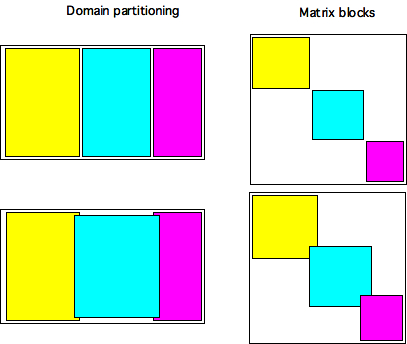
\includegraphics[scale=.6]{bjacobi}
  \caption{Illustration of block Jacobi and Additive Schwarz preconditioners}
  \label{fig:bjacobi}
\end{figure}
Figure~\ref{fig:bjacobi} illustrates these preconditioners both in
matrix and subdomain terms.

\Level 3 {Multigrid preconditioners}

\begin{itemize}
\item There is a native \ac{AMG} type: \indexpetscdef{PCGAMG};
\item the external packages \indexterm{Hypre} and \indexterm{ML} have
  \ac{AMG} methods.
\item There is a general \ac{MG} type: \indexpetscdef{PCMG}.
\end{itemize}

\Level 3 {Field split preconditioners}
\label{sec:pcfieldsplit}

For background refer to section~\ref{sec:matfieldsplit}.

\Level 1 {Customization: monitoring and convergence tests}

PETSc solvers can do various \indexterm{callback}s to user functions.

\Level 3 {Shell preconditioners}

You already saw that,
in an iterative methods, the coefficient matrix can be given operationally
as a \indextermbus{shell}{matrix}; section~\ref{sec:mat-shell}.
Similarly, the preconditioner matrix can be specified operationally
by specifying type \indexpetscdef{PCSHELL}.

This needs specification of the application routine
through \indexpetscdef{PCShellSetApply}:
\begin{lstlisting}
PCShellSetApply(PC pc,PetscErrorCode (*apply)(PC,Vec,Vec));
\end{lstlisting}
and probably specification of a context pointer through
\indexpetscdef{PCShellSetContext}:
\begin{lstlisting}
PCShellSetContext(PC pc,void *ctx);
\end{lstlisting}
The application function then retrieves this context with
\indexpetscdef{PCShellGetContext}:
\begin{lstlisting}
PCShellGetContext(PC pc,void **ctx);
\end{lstlisting}

If the shell preconditioner requires setup, a~routine for this can be specified with
\indexpetscdef{PCShellSetSetUp}:
\begin{lstlisting}
PCShellSetSetUp(PC pc,PetscErrorCode (*setup)(PC));
\end{lstlisting}

\Level 3 {Combining preconditioners}

It is possible to combine preconditioners with \indexpetscdef{PCCOMPOSITE}
\begin{lstlisting}
PCSetType(pc,PCCOMPOSITE);
PCCompositeAddPC(pc,type1);
PCCompositeAddPC(pc,type2);
\end{lstlisting}
By default, the preconditioners are applied additively;
for multiplicative application
\begin{lstlisting}
PCCompositeSetType(PC pc,PCCompositeType PC_COMPOSITE_MULTIPLICATIVE);
\end{lstlisting}

\Level 2 {Convergence tests}

For instance, you can set your own convergence test with
\indexpetscdef{KSPSetConvergenceTest}.
\begin{lstlisting}
KSPSetConvergenceTest
   (KSP ksp,
    PetscErrorCode (*test)(
        KSP ksp,PetscInt it,PetscReal rnorm,
        KSPConvergedReason *reason,void *ctx),
    void *ctx,PetscErrorCode (*destroy)(void *ctx));
\end{lstlisting}
This routines accepts 
\begin{itemize}
\item the custom stopping test function,
\item a `context' void pointer to pass information to the tester, and
\item optionally a custom destructor for the context information.
\end{itemize}
By default, PETSc behaves as if this function has been called with
\indexpetscdef{KSPConvergedDefault} as argument.

\Level 2 {Convergence monitoring}

There is also a callback for monitoring each iteration.
It can be set with \indexpetscdef{KSPMonitorSet}.
\begin{lstlisting}
KSPMonitorSet
   (KSP ksp,
    PetscErrorCode (*mon)(
        KSP ksp,PetscInt it,PetscReal rnorm,void *ctx),
    void *ctx,PetscErrorCode (*mondestroy)(void**));
\end{lstlisting}
By default no monitor is set, meaning that the iteration process
runs without output.
The option \indexpetscoption{ksp_monitor} activates printing
a norm of the residual.
This corresponds to setting \indexpetscdef{KSPMonitorDefault}
as the monitor.

This actually outputs the `preconditined norm' of the residual,
which is not the L2 norm, but the square root of~$r^tM\inv r$,
a~quantity that is computed in the course of the iteration process.
Specifying \indexpetscdef{KSPMonitorTrueResidualNorm}
(with corresponding option \indexpetscoption{ksp_monitor_true_residual})
as the monitor prints the actual norm~$\sqrt{r^tr}$.
However, to compute this involves extra computation,
since this quantity is not normally computed.

\Level 2 {Auxiliary routines}

\indexpetscdef{KSPGetSolution}
\indexpetscdef{KSPGetRhs}
\indexpetscdef{KSPBuildSolution}
\indexpetscdef{KSPBuildResidual}
\begin{lstlisting}
KSPGetSolution(KSP ksp,Vec *x);
KSPGetRhs(KSP ksp,Vec *rhs);
KSPBuildSolution(KSP ksp,Vec w,Vec *v);
KSPBuildResidual(KSP ksp,Vec t,Vec w,Vec *v);
\end{lstlisting}

\Level 0 {Direct solvers}
\label{sec:petsc-direct}

PETSc has some support for direct solvers, that is, variants of LU
decomposition. In a sequential context, the \lstinline{PCLU}
preconditioner can be use for this: a direct solver is equivalent to
an iterative method that stops after one preconditioner
application. This can be forced by specifying a KSP type of
\lstinline{KSPPREONLY}.

Distributed direct solvers are more complicated. PETSc does not have
this implemented in its basic code, but it becomes available by
configuring PETSc with the
\indexterm{scalapack} library.

You need to specify which package provides the LU factorization:

\begin{lstlisting}
PCFactorSetMatSolverType(pc, <solvertype> )
\end{lstlisting}

where solvertype can be mumps, superlu, umfpack, or a number of
others. Note that availability of these packages depends on how PETSc
was installed on your system.

\Level 0 {Control through command line options}

From the above you may get the impression that there are lots of calls
to be made to set up a PETSc linear system and solver. And what if you
want to experiment with different solvers, does that mean that you
have to edit a whole bunch of code? Fortunately, there is an easier
way to do things. If you call the routine
%
\indexpetscref{KSPSetFromOptions}
with the \lstinline{solver} as argument,
%
PETSc will look at your command line options and take those into
account in defining the solver. Thus, you can either omit setting
options in your source code, or use this as a way of quickly
experimenting with different possibilities. Example:

\begin{verbatim}
myprogram -ksp_max_it 200 \
    -ksp_type gmres -ksp_type_gmres_restart 20  \
    -pc_type ilu -pc_type_ilu_levels 3
\end{verbatim}

